\documentclass[conference]{IEEEtran}
\IEEEoverridecommandlockouts
% The preceding line is only needed to identify funding in the first footnote. If that is unneeded, please comment it out.
\usepackage{cite}
\usepackage{amsmath,amssymb,amsfonts}
\usepackage{graphicx}
\usepackage{textcomp}
\usepackage{xcolor}
\usepackage[hidelinks]{hyperref}

\usepackage{makecell} % For wrapping text in cells

\usepackage{graphicx} % For resizing the table

\def\BibTeX{{\rm B\kern-.05em{\sc i\kern-.025em b}\kern-.08em
    T\kern-.1667em\lower.7ex\hbox{E}\kern-.125emX}}
\begin{document}

\title{Second-Life Battery Systems: Exploring Profit Distribution Models and Economic Viability\\
}

\author{\IEEEauthorblockN{1\textsuperscript{st} Shahriar Kariman }
\IEEEauthorblockA{\textit{dept. Electrical Engineering and Computer Science} \\
\textit{University of New Brunswick}\\
Fredericton, Canada \\
skariman@unb.ca}
\and
\IEEEauthorblockN{2\textsuperscript{nd} Promise Eskor Ononokpono}
\IEEEauthorblockA{\textit{dept. Electrical Engineering and Computer Science} \\
\textit{University of New Brunswick}\\
Fredericton, Canada \\
promise.ononokpono@unb.ca}
}

\maketitle

\begin{abstract}

As the  adoption of electric vehicles (EVs) accelerates, managing end-of-life EV batteries has become a pressing challenge.  As battery recycling remains costly, repurposing these batteries for second-life applications presents an economically viable and sustainable alternative. Current second-life battery businesses primarily acquire ownership of end-of-life batteries through partnerships, purchases, or government support. In this paper, we propose an alternative business model where individual EV owners retain battery ownership and receive a share of the profits generated through battery reuse. To facilitate this, we present and simulate  two profit distribution approaches: one based on real-time battery performance tracking and another using a more static state-of-health (SOH)-based model.

The arbitrage simulation, spanning 10 years, compares these approaches against an individual battery baseline using real-world energy pricing data and battery degradation models. Our results show that cluster-based energy storage outperforms individual battery systems, generating higher profits while better preserving battery SOH. Among the proposed profit-sharing models, Model 1 performs best in clusters with similar-strength batteries, whereas Model 2 provides fairer profit distribution for clusters with varied-strength batteries.

These findings demonstrate the economic potential of a profit-sharing second-life battery business and highlight practical implications for profit optimization. Future research can further enhance these results by integrating additional revenue streams, such as demand response programs, and optimizing cluster management strategies for increased profitability.

\end{abstract}

\begin{IEEEkeywords}
Electric vehicles (EVs), Second-life batteries, Battery recycling, Battery repurposing,
Profit-sharing model, Battery state of health (SOH), Energy storage, Arbitrage simulation,
Sustainable business models
\end{IEEEkeywords}

\section{Introduction}

With the global transition towards renewable energy and electric vehicles, the demand for lithium-ion batteries is on the rise \cite{b1}. While EV batteries will no longer be able to be used for transportation after reaching 70-80\% of their original battery capacity \cite{b2}. And because EV battery recycling is still very expensive, their reuse is considered to be a more lucrative option as such EV companies have begun to form partnerships with battery manufactures and recycling companies to develop a market around second-life batteries \cite{b3}.

\section{Background}

One of the key factors for a second-life business model is the battery ownership meaning who owns the batteries and decides on the management in the resulting second-life energy system. Currently in most businesses batteries are often obtained through inter-industry partnerships and with government support \cite{b4}.

For a better understanding of the current industry methods with regards to acquiring batteries we looked at 3 successful companies utilizing second-life battery reuse to create a circular economy for batteries.

\begin{table}[htbp]
\caption{Examples of Businesses Utilizing  Second-life}
\begin{center}
\begin{tabular}{|c|c|c|c|}
\hline
\textbf{Company} & \textbf{Business Model} & \textbf{Based In} \\ \hline
Zenobe & EV Manufacturing Company & London \\ \hline
Modual & Battery Repurposing & Switzerland \\ \hline
ECO STORE & Energy Storage Manufacturing Company & Norway \\ \hline
\end{tabular}
\end{center}
\end{table}

All 3 of these companies repurpose used batteries for different second-life applications but they differ in the means of acquiring them, from direct reuse of their own products to partnerships with recycling businesses and government support.

\begin{itemize}
  \item Zenobe reuses end of life batteries from their manufactured electric buses, trucks and commercial vehicles currently in operation \cite{b5}.
  \item Modual purchases batteries and repurposes them for resale in home and business applications \cite{b6}. They also recently secured financing from Switzerland’s Technology Fund to help with their effort \cite{b7}.
  \item ECO STORE acquires the second-life batteries it uses alongside their first-life batteries through their partnership with Morrow and Li-Cycle Holdings which is another battery recycling business \cite{b8, b9}.
\end{itemize}

\subsection{Another Approach}

So far from our research we have established that second-life battery companies have ownership of the batteries they use either as a by-product of their business model or acquire them through transactions and partnerships. We have yet to encounter a case where a business does not own the batteries directly and essentially partners with individual EV owners to reuse their end of life batteries for a cut of the profits, effectively making them shareholders of the business.

But in order for such a business to exist there needs to be an effective and clear way to distribute the profit from the batteries between the business and the battery owners. This is to ensure transparency and trust between all parties involved and satisfaction from the end result.

We propose two potential approaches to profit distribution for such a business:

\begin{enumerate}
    \item The batteries put together in a cluster could have a system alongside them that continuously gathers information on the batteries charge and discharge along with their state of health. That way the contribution of each battery can be definitively calculated and a share of the revenue sent back to the owner.
    \item The batteries could be checked at the beginning and based on the state of health and capacity of the battery assigned a percentage that the owners will receive from the entire cluster. This percentage continues to adjust based on the state of health and capacity of the battery over the course of the simulation.
\end{enumerate}

We aim to model these 2 scenarios to find out which is more profitable and easier to
implement. We hope to shed some light on how a second life battery company should operate
without partnership with other industries or tracking and buying a large number of batteries.

\section{Simulation Design}

For the simulation we assumed that a second-life battery storage system or cluster has 32 batteries. And at the beginning of the simulation we assumed each battery will have an original capacity between 30 to 50 kWh and an initial state of health(SOH) of 60 to 80\% with both capacity and SOH generated randomly.

\begin{equation}
	SOH = \frac{current \ capacity}{original \ capacity}
\end{equation}

In the simulation loop we simulate the use of the batteries for arbitrage over a period of 10 years once for each battery individually and once as all of them managed as part of a storage system of 32 batteries. The arbitrage simulation uses the TOU rates obtained from the Ontario Energy Board \cite{b11}.

For the batteries in the storage system we used a greedy algorithm to distribute the load for each one hour period meaning we sorted the batteries in descending order of state of health and in ascending or descending order of state of charge depending on whether the cluster is charging or discharging.

And based on the outcome of the greedy algorithm we calculated the cycle degradations and calendar degradations using formulas found in an IEEE paper titled “Joint Arbitrage and Operating Reserve Scheduling of Energy Storage Through Optimal Adaptive Allocation of the State of Charge” by Hadi Khani and Hany E. Z. Farag from York University of Toronto \cite{b10}.

Here are the formulas we used to calculate the degredations:

\begin{equation}
\begin{aligned}
	D_{cycle} = K_{cycle} \times \frac{| \Delta E |}{current \ capacity}
\end{aligned}
\end{equation}

\begin{equation}
\begin{aligned}
	D_{calender} = K_{calender} \times \Delta{T}
\end{aligned}
\end{equation}

Where:
\begin{itemize}
    \item \( D_{cycle} \) is the cycle degredation for an hour,
    \item \( D_{calender} \) is the calender degredation for T hours,
    \item \( K_{cycle} \) is the cycle degredation rate per full charge rate equal to $ 4.6 \times 10^{-3}$ , and
    \item \( K_{calender} \) represents the time based degredation rate per hour assuming 2\% annual degredation.
\end{itemize}

After having the degradations the simulation then re-calculates the current capacity based on the same IEEE paper used to calculate the degradations \cite{b10}.

\begin{equation}
\begin{aligned}
	new \ capacity = capacity - total \ degredation
\end{aligned}
\end{equation}

The entire simulation is implemented with object oriented programming principles in mind and it comprises of four main classes for running the simulation as well as some pytests to test the functionality of “battery.py”, “cluster.py” and the decision making algorithm used in “arbitrage\_simulation.py”. Figure 1 shows a class diagram of the simulation.

\begin{figure}[h!]
    \centering
    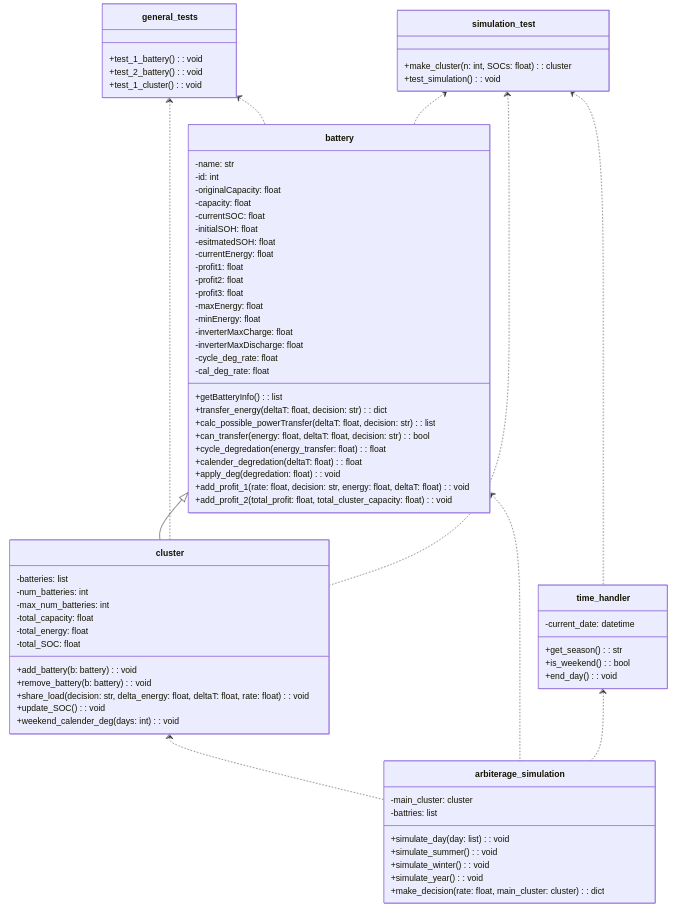
\includegraphics[width=0.5\textwidth]{{img/class_diagram.png}}
    \caption{Class diagram for the simulation.}
    \label{fig:class diagram}
\end{figure}

At the end the simulation results are stored within the battery objects, analyzed using NumPy, and visualized with Plotly.

\section{Simulation Results}

In this section, we will discuss and analyze the results of our simulations using tables and plots. As stated earlier, over  the 10 years of arbitrage simulations, we kept track of the profits and SOH of the cluster distribution models and the individual battery arbitrage models. The values were then compiled annually. These yearly averages are what we will consider here.The purpose of presenting these results is to compare the differences between our two cluster profit distribution models, but also to consider if the cluster has any advantages over an individual arbitrage simulation.

\subsection{Overall Cluster Analysis (Profitability and State of Health Dynamics)}

Table 2 presents a summary of total profits and SOH reduction for both cluster and individual battery arbitrage simulations. Since cluster generation is random for every run, the values in Table 2 represent the average of 11 simulations. The cluster models achieved the higher total profits, outperforming the individual arbitrage model by 4.6\%. The cluster was again better at retaining the SOH of the batteries, albeit very minimal.

\begin{table}[htbp]
\caption{Comparison of Models Based on Profits and SOH Decrease}
\begin{center}
\resizebox{0.5\textwidth}{!}{
\begin{tabular}{|c|c|c|c|}
\hline
\textbf{Models} & \textbf{Total Profits (\$)} & \textbf{\makecell{SOH Decrease (\%) }} & \textbf{\makecell{Average SOH (\%) }} \\ \hline
Cluster Models & 76,847 & 55.6\% & 39.95\% \\ \hline
Individual Arbitrage Model & 73,300 & 56.4\% & 40.33\% \\ \hline
\end{tabular}
}
\end{center}
\end{table}

\subsection{Individual Profitability Analysis}

Previously, we looked at the results of the simulation from a group perspective. Here, we look at the same results but from an individual battery standpoint. Table 3 contains the information of the cluster that we are going to analyse.

\begin{table}[htbp]
\caption{Battery Information: Capacity and SOH}
\begin{center}
\resizebox{0.5\textwidth}{!}{
\begin{tabular}{|c|c|c|c|c|}
\hline
\textbf{Name} & \textbf{ID} & \textbf{Original Capacity (kWh)} & \textbf{Starting Capacity (kWh)} & \textbf{Initial SOH (\%)} \\ \hline
Battery\_1 & 0 & 37 & 22.36 & 60 \\ \hline
Battery\_2 & 1 & 39 & 30.39 & 78 \\ \hline
Battery\_3 & 2 & 44 & 33.92 & 77 \\ \hline
Battery\_4 & 3 & 34 & 25.64 & 75 \\ \hline
Battery\_5 & 4 & 42 & 30.08 & 72 \\ \hline
Battery\_6 & 5 & 49 & 36.23 & 74 \\ \hline
Battery\_7 & 6 & 39 & 24.89 & 64 \\ \hline
Battery\_8 & 7 & 32 & 19.86 & 62 \\ \hline
Battery\_9 & 8 & 39 & 30.47 & 78 \\ \hline
Battery\_10 & 9 & 39 & 23.64 & 61 \\ \hline
Battery\_11 & 10 & 50 & 31.39 & 63 \\ \hline
Battery\_12 & 11 & 36 & 24.98 & 69 \\ \hline
Battery\_13 & 12 & 39 & 28.60 & 73 \\ \hline
Battery\_14 & 13 & 50 & 39.69 & 79 \\ \hline
Battery\_15 & 14 & 37 & 27.19 & 73 \\ \hline
Battery\_16 & 15 & 30 & 18.11 & 60 \\ \hline
Battery\_17 & 16 & 34 & 23.90 & 70 \\ \hline
Battery\_18 & 17 & 45 & 27.32 & 60 \\ \hline
Battery\_19 & 18 & 42 & 29.75 & 71 \\ \hline
Battery\_20 & 19 & 36 & 26.85 & 75 \\ \hline
Battery\_21 & 20 & 34 & 21.73 & 64 \\ \hline
Battery\_22 & 21 & 40 & 26.14 & 65 \\ \hline
Battery\_23 & 22 & 44 & 32.82 & 75 \\ \hline
Battery\_24 & 23 & 48 & 29.00 & 60 \\ \hline
Battery\_25 & 24 & 46 & 32.99 & 72 \\ \hline
Battery\_26 & 25 & 39 & 28.29 & 73 \\ \hline
Battery\_27 & 26 & 41 & 29.73 & 73 \\ \hline
Battery\_28 & 27 & 35 & 27.70 & 79 \\ \hline
Battery\_29 & 28 & 35 & 26.92 & 77 \\ \hline
Battery\_30 & 29 & 46 & 33.75 & 73 \\ \hline
Battery\_31 & 30 & 50 & 36.02 & 72 \\ \hline
Battery\_32 & 31 & 38 & 26.98 & 71 \\ \hline
\end{tabular}
}
\end{center}
\end{table}

\begin{itemize}
  \item Cluster Profit Model 1: As illustrated in Fig. 2, this distribution model generates the highest profit for 50\% of the batteries. However, in cases where it does not perform best, it tends to be the worst-performing model. This trend remained consistent across all simulations. The model’s reliance on higher battery utilization for increased profits likely explains its varied performance, as stronger batteries are disproportionately used compared to weaker ones in our cluster system.
  \item Cluster Profit Model 2: Model 2 demonstrates strong and consistent performance, as shown in Fig. 2. It generates the highest profit for 50\% of the batteries and, in situations where it does not perform best, it consistently ranks as the second-best model. Notably, this model also achieves the highest individual profit for a single battery. This outcome aligns with expectations, as profits are distributed based on fixed percentages, ensuring each battery earns a share regardless of its contribution. These observations were consistent across all simulations.

  \item Single User Profit (Individual Arbitrage Model): The individual arbitrage model consistently underperforms relative to the cluster-based models, ranking as the worst-performing approach for over 50\% of the batteries. Additionally, it never achieved the highest profit for any individual battery. This shortcoming arises because the individual arbitrage model generates lower profits compared to cluster-based management, where collective operation enables greater economic potential.
\end{itemize}

\begin{figure}[h!]
    \centering
    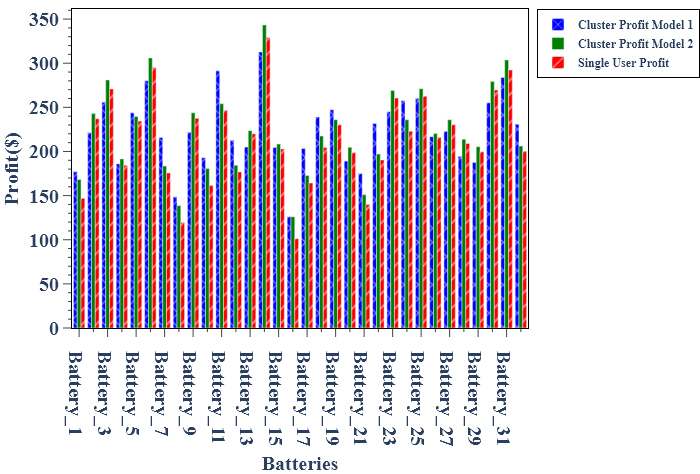
\includegraphics[width=0.5\textwidth]{{img/average_yearly_profit.png}}
    \caption{Average Yearly Profit.}
    \label{fig: Average Yearly Profit}
\end{figure}

\subsection{Individual State of Health (SOH) Dynamics}

Fig. 3 and Fig. 4 depict the state of health (SOH) dynamics from an individual battery perspective and a group perspective, respectively. These figures allow us to draw general inferences about the behavior observed in the simulations. Although the results presented are from a single simulation, the trends remained consistent across all simulations conducted.

The SOH decline throughout the simulation is largely similar for both the cluster and individual arbitrage models. However, when discrepancies occur, the cluster model typically exhibits a lower rate of SOH degradation. This is likely due to the cluster's ability to distribute the load across multiple batteries, resulting in reduced wear and tear per battery on average.

\begin{figure}[h!]
    \centering
    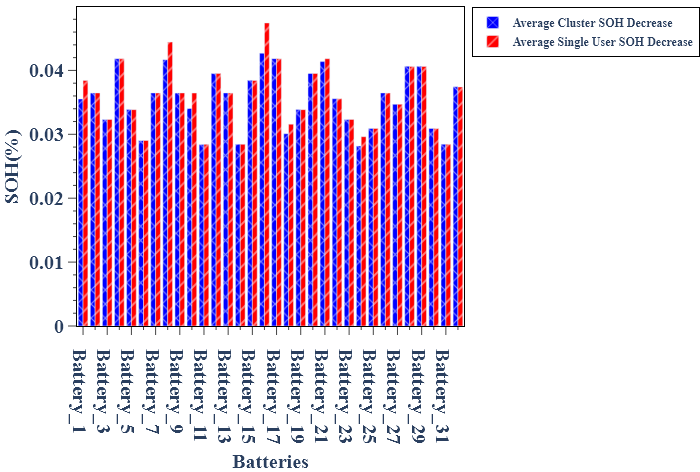
\includegraphics[width=0.5\textwidth]{{img/average_yearly_SOH_decrease.png}}
    \caption{Average Yearly  State of Health Decrease.}
    \label{fig: Average Yearly  State of Health Decrease}
\end{figure}

\begin{figure}[h!]
    \centering
    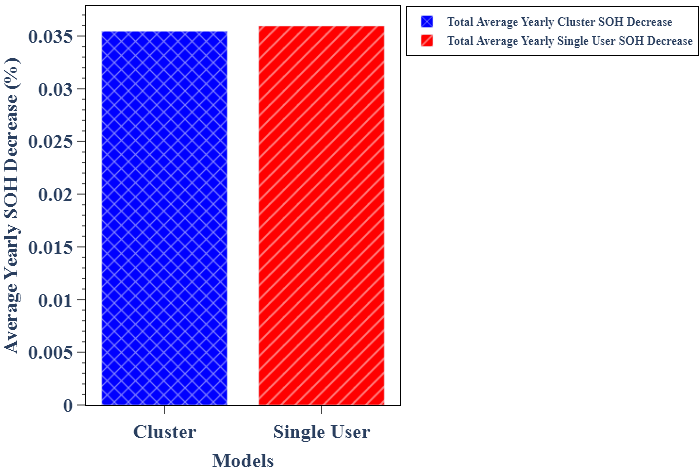
\includegraphics[width=0.5\textwidth]{{img/average_yearly_soh_decrease_group.png}}
    \caption{Average Yearly  State of Health Decrease.}
    \label{fig: Average Yearly  State of Health Decrease}
\end{figure}

\subsection{Trend Analysis}

We will look a bit more into the results to analyze the trends in average yearly profit based on the state of health and the capacity of the batteries.

\begin{itemize}
  \item Cluster Profit Model 1: As shown in Fig. 5, there is a slight positive correlation between the average yearly profit and the initial SOH in Cluster Profit Model 1. This supports our earlier observation that stronger batteries are utilized more intensively. Fig. 6 further highlights that starting capacity plays a significant role in determining what qualifies as a "stronger" battery. This results in a clear positive correlation between a battery's starting capacity and its profit generation.
  \item Cluster Profit Model 2: In Fig. 7, a much more pronounced positive correlation between the average yearly profit and the initial SoH is evident compared to Model 1. This result is consistent with our expectations, as the SOH directly influences the percentage-based profit distribution in Cluster Profit Model 2. Additionally, Fig. 8 shows an almost linear relationship between starting capacity and profit. This is likely due to the interplay between SoH and capacity (capacity = SOH * Original Capacity), with higher capacity significantly impacting the profit-sharing mechanism among stakeholders.
\end{itemize}

\begin{figure}[h!]
    \centering
    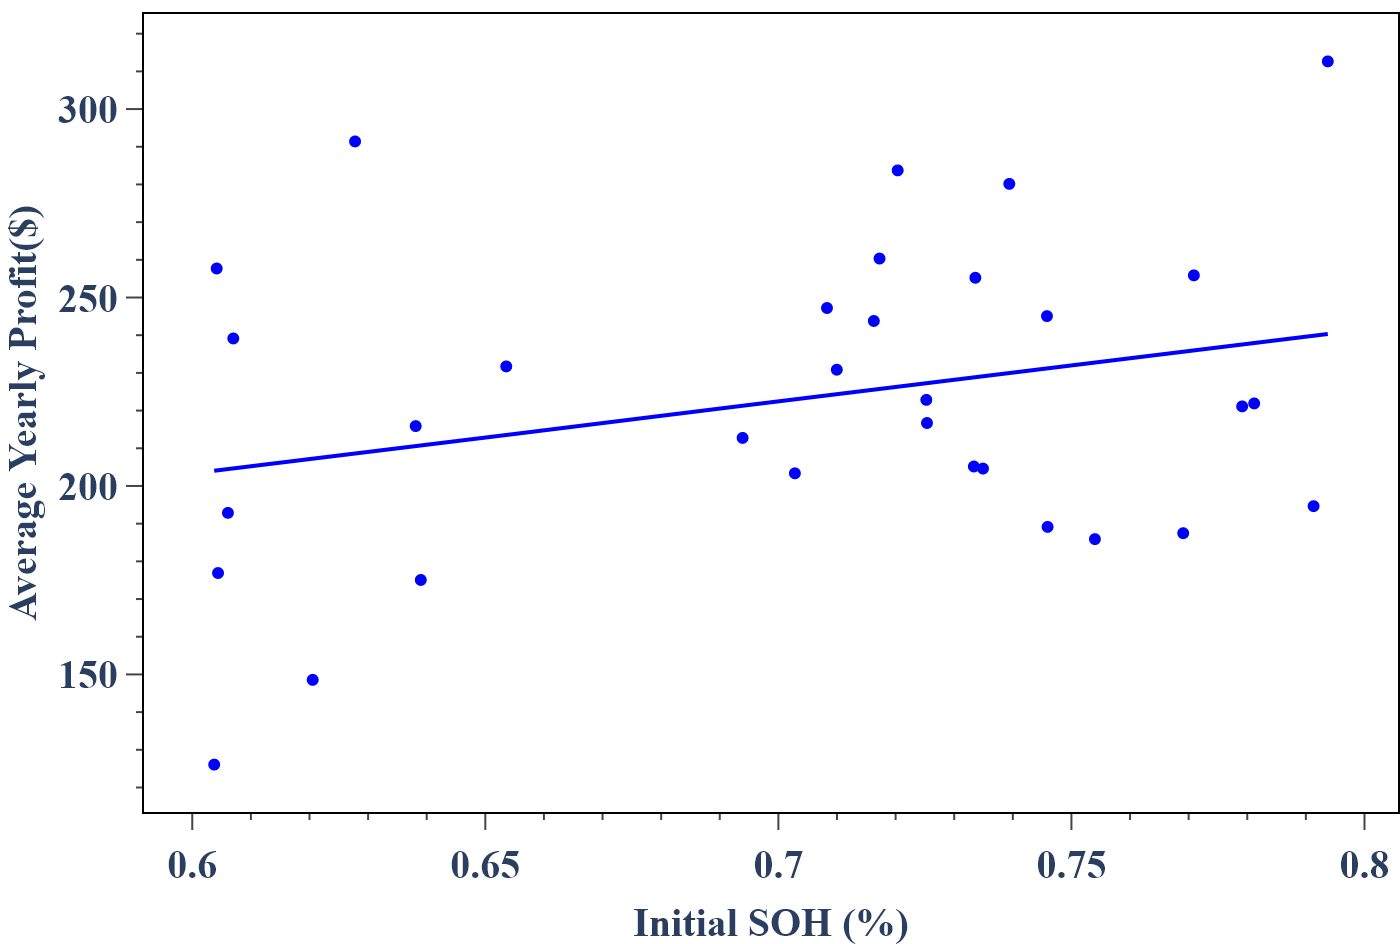
\includegraphics[width=0.5\textwidth]{{img/initialSOH+vs_Average_Yearly_Profit (Model 1, $).png}}
    \caption{Initial SOH (\%) vs. Average Yearly Profit (Model 1, \$) }
    \label{fig: Initial SOH vs.  Average Yearly Profit 1}
\end{figure}

\begin{figure}[h!]
    \centering
    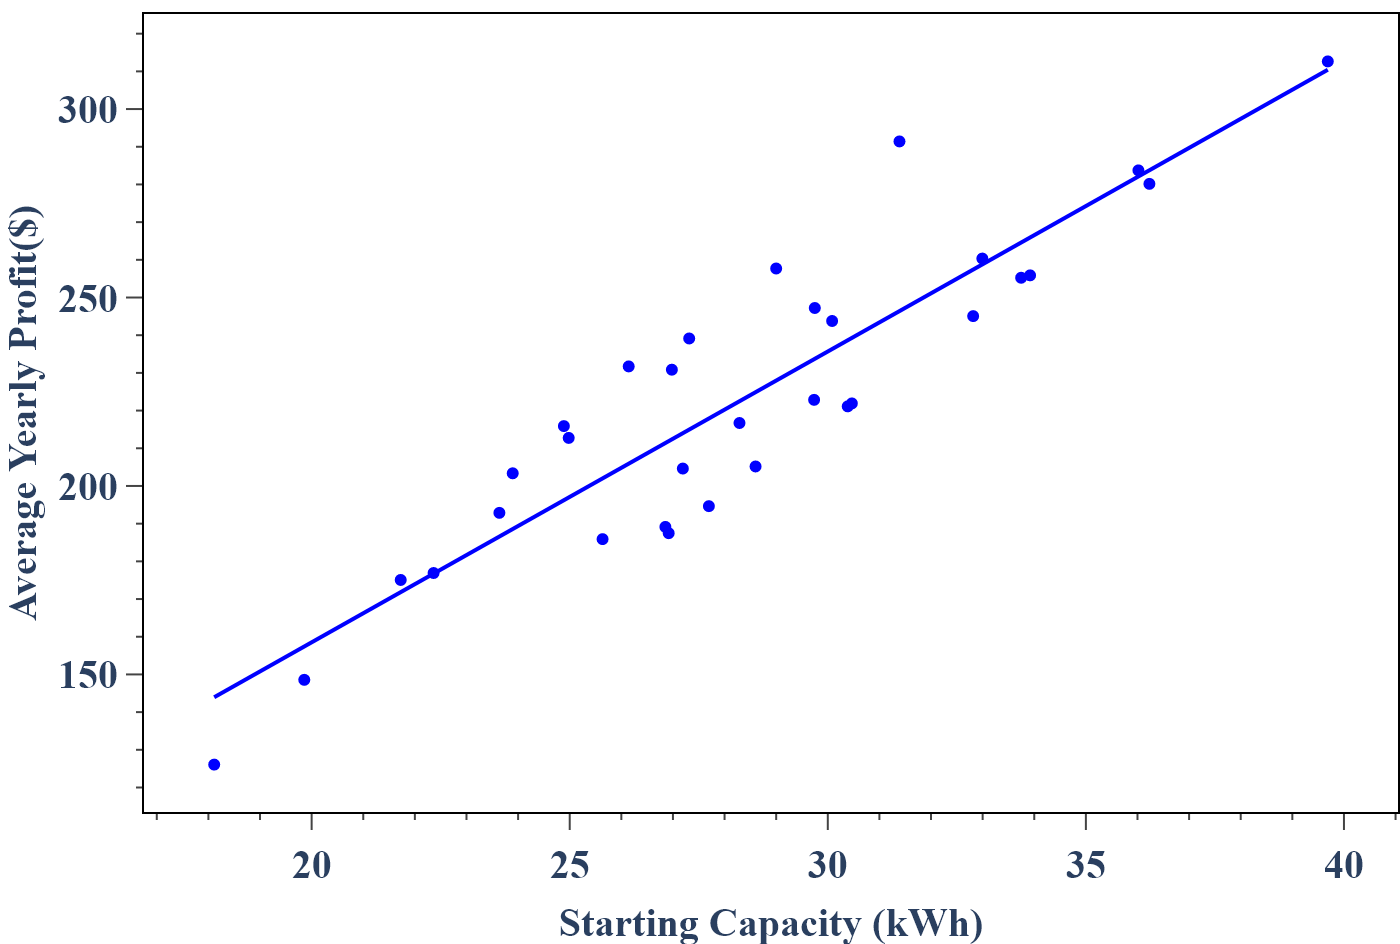
\includegraphics[width=0.5\textwidth]{{img/startingCapacityvsAverage Yearly Profit (Model 1, $).png}}
    \caption{Starting Capacity(kWh) vs. Average Yearly Profit (Model 1, \$) }
    \label{fig: Starting Capacity vs.  Average Yearly Profit 1}
\end{figure}

\begin{figure}[h!]
    \centering
    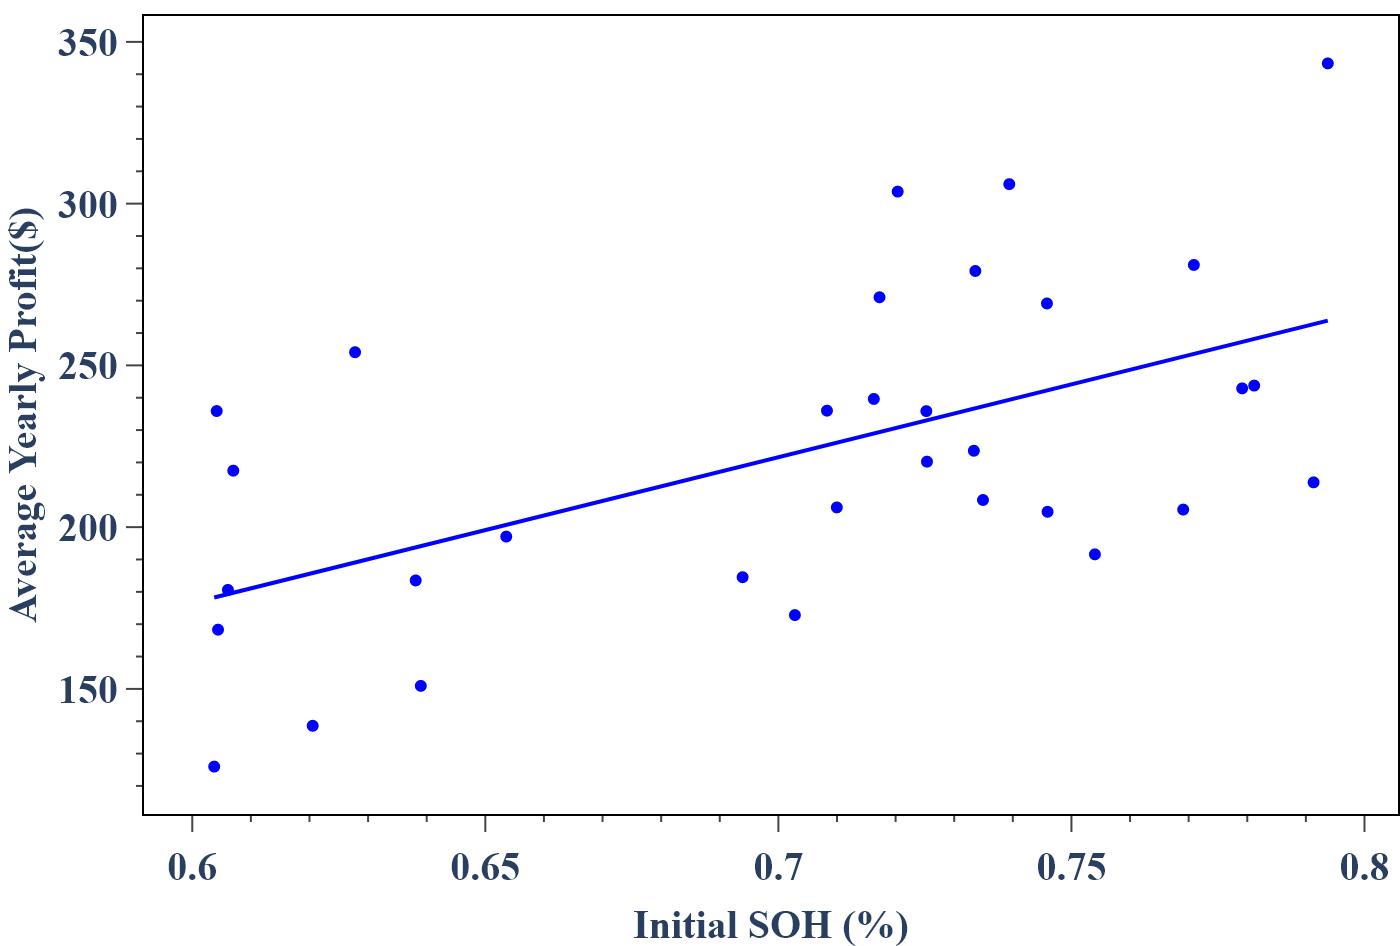
\includegraphics[width=0.5\textwidth]{{img/initialSOHvsAverage Yearly Profit (Model 2, $).png}}
    \caption{Initial SOH (\%) vs. Average Yearly Profit (Model 2, \$) }
    \label{fig: Initial SOH vs.  Average Yearly Profit 2}
\end{figure}

\begin{figure}[h!]
    \centering
    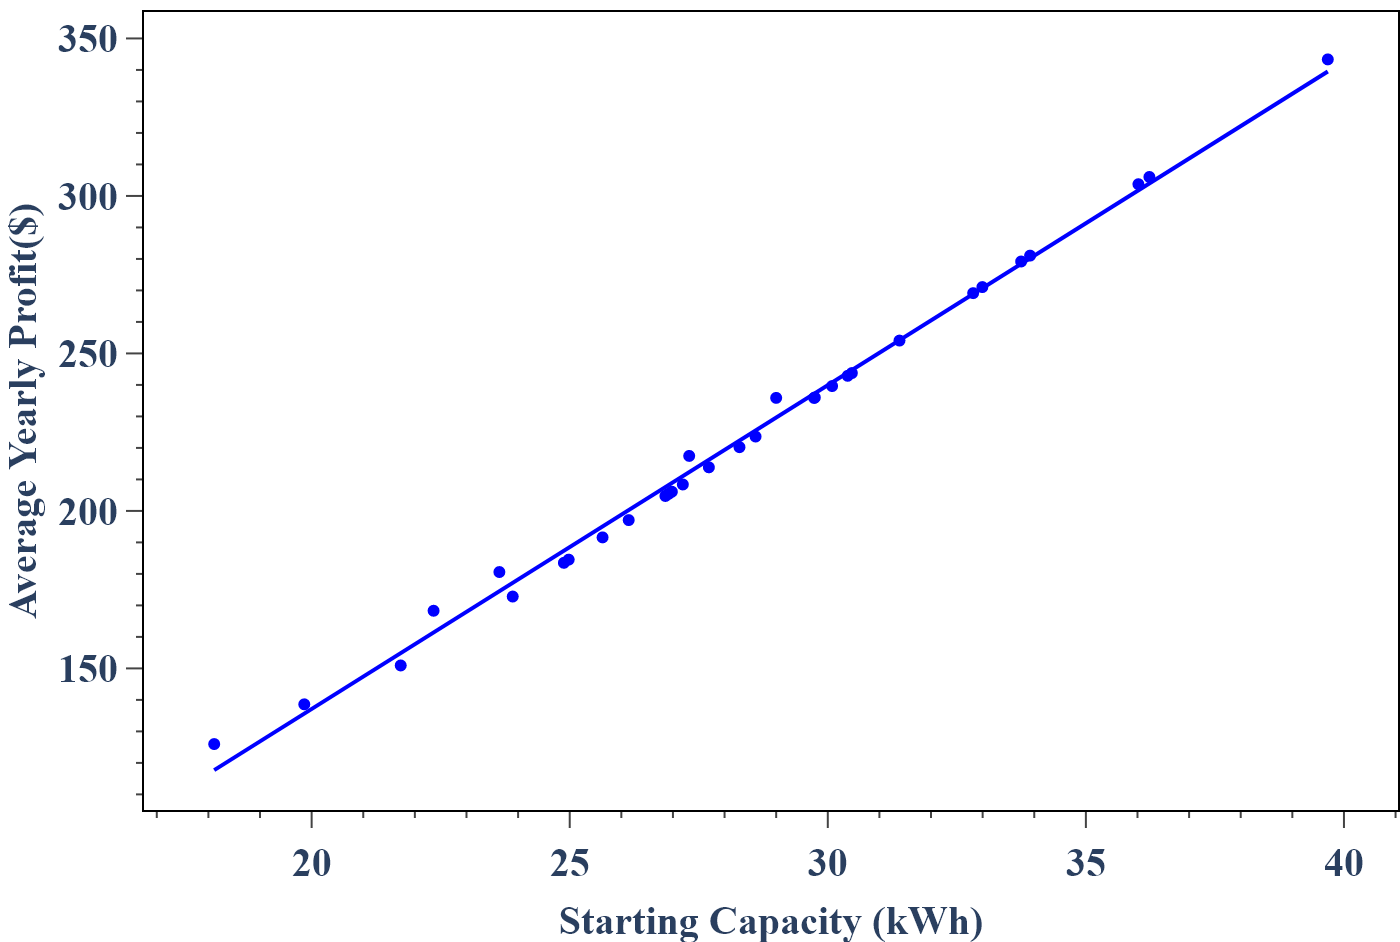
\includegraphics[width=0.5\textwidth]{{img/startingCapacityvsAverage Yearly Profit (Model 2, $).png}}
    \caption{Starting Capacity(kWh) vs. Average Yearly Profit (Model 2, \$) }
    \label{fig: Starting Capacity vs.  Average Yearly Profit 2}
\end{figure}

\subsection{Comparative Insights}

The results suggest that cluster profit model 2 offers a more equitable distribution of profit in clusters with significant disparities in battery strength. This is because it provides a more stable spread of profit among clients. In this model, the weaker batteries generate the most profit compared to the other two models. In a cluster where the batteries are relatively uniform in strength, model 1 would produce a similar profit spread, with a slight preference toward the higher-contributing batteries. In this case, the batteries would exhibit more equal usage across the cluster. Finally, the cluster model is more profitable than the individual arbitrage model, while also being slightly better at preserving the state of health of the batteries.

\subsection{Practical Implications}

These findings hold important implications for stakeholders in the second-life EV battery industry. Cluster model 1 should be implemented in clusters with similar battery strength to ensure more even profit distribution among stakeholders. On the other hand, cluster model 2 should be applied in clusters with greater variance in battery strength, as it better supports weaker batteries. A business could potentially combine both models, using them on a cluster composition basis for an optimal approach.

\section{Conclusion}

Currently the business involving batteries acquire ownership of their end of life batteries through purchasing with the help of industry partnerships and government support. Alternatively a second-life battery business would be to partner with individual EV owners for a share of the profit their battery could generate.

In this paper we simulated such a business model where the batteries are grouped together for arbitrage compared to the base case where each individual battery is used separately. We also proposed 2 different profit distribution methods for the resulting battery system to get an insight to the more appealing profit distribution approach.

We found that the cluster-based approach generates higher profits compared to the sum of individual battery profits. Among the profit distribution models in the cluster, Model 1 performs a more even distribution for clusters with equal-strength battery compositions, whereas Model 2 demonstrates superior distribution in clusters with varied-strength battery compositions.

While the arbitrage simulations revealed a notable profit advantage, there remains significant untapped income potential. Integrating our system with complementary programs, such as demand response, could substantially enhance earnings. Additionally, further optimizations to the cluster management system are expected to yield even greater profit margins.

Future research could explore these avenues, along with other influencing factors not considered in this study, such as the cost of system implementation and the business share of profits.

\section*{Acknowledgment}

The authors, Shahriar Kariman\textsuperscript{1} and Promise Eskor Ononokpono\textsuperscript{2}, contributed equally to this work.

\begin{thebibliography}{00}
\bibitem{b1} Q. Hassan, P. Viktor, T. J. Al-Musawi, B. M. Ali, S. Algburi, H. M. Alzoubi, A. Khudhair Al-Jiboory, A. Z. Sameen, H. M. Salman, and M. Jaszczur, ``The renewable energy role in the global energy transformations,'' \textit{Renewable Energy Focus}, vol. 48, p. 100545, 2024. [Online]. Available: \href{https://www.sciencedirect.com/science/article/abs/pii/S1755008424000097?casa_token=bUNZr0M6nogAAAAA:BW6rOq1yhF3iUOtobThX-tDWVjZDpJL9Hzmk0HS78usaDj24Zq_MftqZLBkgYpIrtdgdilaX}{www.sciencedirect.com/science/article/abs/pii/S1755008424000097}.

\bibitem{b2} A. Keeli and R. K. Sharma, ``Optimal use of second life battery for peak load management and improving the life of the battery,''  \textit{2012 IEEE International Electric Vehicle Conference}, Greenville, SC, USA, 2012, pp. 1--6. doi: \href{https://ieeexplore-ieee-org.proxy.hil.unb.ca/document/6183276}{ieeexplore-ieee-org.proxy.hil.unb.ca/document/6183276}.


\bibitem{b3} Y. Zhao, O. Pohl, A. I. Bhatt, G. E. Collis, P. J. Mahon, T. Rüther, and A. F. Hollenkamp, ``A review on battery market trends, second-life reuse, and recycling,'' \textit{Sustainable Chemistry}, vol. 2, no. 1, pp. 167--205, 2021. doi: \href{https://www.mdpi.com/2673-4079/2/1/11}{www.mdpi.com/2673-4079/2/1/11}.

\bibitem{b4} N. Jiao and S. Evans, ``Business models for sustainability: The case of second-life electric vehicle batteries,'' \textit{Procedia CIRP}, vol. 40, pp. 250--255, 2016. [Online]. Available: \href{https://www.sciencedirect.com/science/article/pii/S2212827116001293}{www.sciencedirect.com/science/article/pii/S2212827116001293}.

\bibitem{b5} Zenobe Energy [Online]. Available: \href{https://www.zenobe.com/our-story/}{www.zenobe.com/our-story/}. [Accessed: Dec. 2024].

\bibitem{b6} Modual, Modual Series Lite [Online]. Available: \href{https://modual.ch/series-lite/}{modual.ch/series-lite/}. [Accessed: Dec. 2024].

\bibitem{b7} Modual, Technology Fund PR [Online]. Available: \href{https://modual.ch/technology-fund-pr/}{modual.ch/technology-fund-pr/}. [Accessed: Dec. 2024].

\bibitem{b8} ECO STOR, Partners [Online]. Available: \href{https://www.eco-stor.com/partners}{www.eco-stor.com/partners}. [Accessed: Dec. 2024].

\bibitem{b9} Li-Cycle and Strategic Partners to Build New Lithium-ion Battery Recycling Facility in Norway, Li-Cycle, Jan. 26, 2022. [Online]. Available: \href{https://investors.li-cycle.com/news/news-details/2022/Li-Cycle--Strategic-Partners-to-Build-New-Lithium-ion-Battery-Recycling-Facility-in-Norway/default.aspx}{https://investors.li-cycle.com/news/news-details/2022/Li-Cycle--Strategic-Partners-to-Build-New-Lithium-ion-Battery-Recycling-Facility-in-Norway/default.aspx}. [Accessed: Dec. 14, 2024].

\bibitem{b10} H. Khani and H. E. Z. Farag, ``Joint Arbitrage and Operating Reserve Scheduling of Energy Storage Through Optimal Adaptive Allocation of the State of Charge,'' \textit{IEEE Trans. Sustainable Energy}, vol. 10, no. 4, pp. 1705--1717, Oct. 2019, doi: \href{https://ieeexplore.ieee.org/document/8463591}{ieeexplore.ieee.org/document/8463591}.

\bibitem{b11}
Ontario Energy Board, ``Electricity rates,'' [Online]. Available: \href{https://www.oeb.ca/consumer-information-and-protection/electricity-rates}{www.oeb.ca/consumer-information-and-protection/electricity-rates}. [Accessed: Dec. 12, 2024].


\end{thebibliography}

\end{document}
